%!TEX root = Slic3r-Manual.tex

\subsection{Simple Mode}
Slic3r has two modes of operation, Simple and Expert. These may be chosen from the \texttt{Preferences} window (found under the \texttt{File} menu).  

\setlength\fboxsep{10pt}
\setlength\fboxrule{0pt}
\noindent
\centerline{\fbox{\includegraphics[width=0.3\textwidth]{simple_mode/preferences_general.png}}}

As is expected, the simple mode offers a cut-down set of options, enough for the beginner to get started with.  The expert options give more control over how Slic3r produces the gcode and will be looked at later.

\subsubsection{Print Settings}

The \texttt{Print Settings} tab provides the opportunity to change settings related to the actual print.  Whereas the other tabs are changed rarely, the settings on this tab will be modified regularly, possibly for each model printed.

\begin{figure}[ht]
\centering
\includegraphics[width=\textwidth]{simple_mode/simple_mode_print_settings.png}
\caption{Simple Mode: Print Settings.}
\label{fig:simple_mode_print_settings}
\end{figure}

\paragraph{General.} % (fold)
\label{par:simple_general}

\texttt{Layer height} of the extrusion is controlled by how much material is pushed from the nozzle and the proximity of the nozzle to the print bed.  There are several factors that influence how high each layer should be:
\begin{itemize}
	\item \textbf{Desired resolution}  - Lower layer height should result in prints with less noticeable ribs or bands, as each layer is smaller.  Aesthetics plays a role here, but also the type of model, for example, a mechanical part may not need such a high resolution finish, whereas a presentation piece may do so.
	\item \textbf{Print speed}  - Shorter layers will result in smoother prints but each print will take longer, simply because the extruder must trace the pattern more times.  A later goal will be to strike a balance between layer height, the speed of the printer, and the quality of the resulting print.
\end{itemize} 

\texttt{Perimeters} defines the minimum number of vertical shells (i.e. walls) a print will have.  Unless the model requires single width walls it is generally recommended to have a minimum of two perimeters as this gives some insurance that if a section of the perimeter is not printed correctly then the second perimeter will help cover it.

The upper and lowermost layers that sandwich the model are filled with a \texttt{Solid layers} pattern.  For the bottom layers the important factor to consider is how the surface will look should there be a mistake whilst laying down the first layer, and for this reason it is recommended to have at least two bottom layers.  Of course, once the printer is reliably producing excellent results this can be reduced, if so desired.

A similar consideration is required for the top layers.  Because the intermediate layers are likely to be filled with a pattern set less than 100\% then the covering layers will have to bridge this pattern and this can require more than one pass to cover completely.

% paragraph general (end)


\paragraph{Infill.} % (fold)
\label{par:simple_infill}
For the majority of cases it makes no sense to 100\% fill the model with plastic, this would be a waste of material and take a long time.  Instead, most models can be filled with less material which is then sandwiched between layers filled at 100\% (see \texttt{Solid layers} above).

Slic3r offers several fill patterns, and these will be discussed in more depth in section \ref{sec:infill_choices}.  Choosing a pattern will depend on the kind of model and personal taste.  The more exotic fill methods are usually too slow and unnecessarily complex for most use cases, and so most of the time the infill pattern is either \texttt{rectilinear}, \texttt{line}, or \texttt{honeycomb}.

% paragraph infill (end)

\paragraph{Support material.} % (fold)
\label{par:simple_support_material}
Printing a model from the bottom up, as with FDM, means that any significant overhangs will be printed in the air, and most likely droop or not print correctly.  Choosing support material will add additional structures around the model which will build up to then support the overhanging part.  The \texttt{Pattern spacing} option determines how dense the support material is printed.

\begin{figure}[H]
\centering
\includegraphics[width=0.75\textwidth]{advanced/support.JPG}
\caption{An example of support material.}
\label{fig:an_example_of_support_material}
\end{figure}

Tip: It is sometimes worth considering altering the orientation of the model in order to possibly reduce overhangs.

\texttt{Raft layers} will add additional layers underneath the model, providing more anchorage for the object on the bed, but also requiring post processing to remove it.
% paragraph support_material (end)

\paragraph{Speed.} % (fold)
\label{par:simple_speed}
In simple mode there are only three speed settings to consider:
\begin{itemize}
	\item \texttt{Perimeters}  - The outline of the model may benefit from being printed slightly slower so that the outside perimeter of the print has fewer blemishes.
	\item \texttt{Infill}  - As the infill is hidden this can be extruded a little faster.  Take care though not to go too fast as higher speeds results in thinner extrusions, and this may affect how the extrusions bond.
	\item \texttt{Travel}  - The jump between the end of one extrusion and the next should usually be performed as quickly as the printer will allow in order to minimise any mess caused by material oozing from the nozzle.
\end{itemize}
% paragraph speed (end)

\paragraph{Brim.} % (fold)
\label{par:simple_brim}
\texttt{Brim} is used to add more perimeters to the first layer in order to provide more surface area for the print to stick (see §\ref{sec:the_important_first_layer}). The brim is then removed once the print is finished and removed from the bed.
% paragraph brim (end)


\paragraph{Sequential printing.} % (fold)
\label{par:simple_sequential_printing}
When printing several objects at once it can be useful to print each one separately as this will minimise oozing and strings running between the prints.  Care has to be taken that the nozzle and extruder does not interfere with already printed parts.  This is the reason for the \texttt{Extruder clearance} parameters: 
\begin{itemize}
	\item \texttt{Radius}  - The clearance that should be given around the extruder.  Take care if the extruder is not mounted centrally - take the largest safe value.
	\item \texttt{Height}  - The vertical distance between the nozzle tip and the X axis rods, or lowest part which may interfere with a finished print.
\end{itemize}

\begin{figure}[H]
\centering
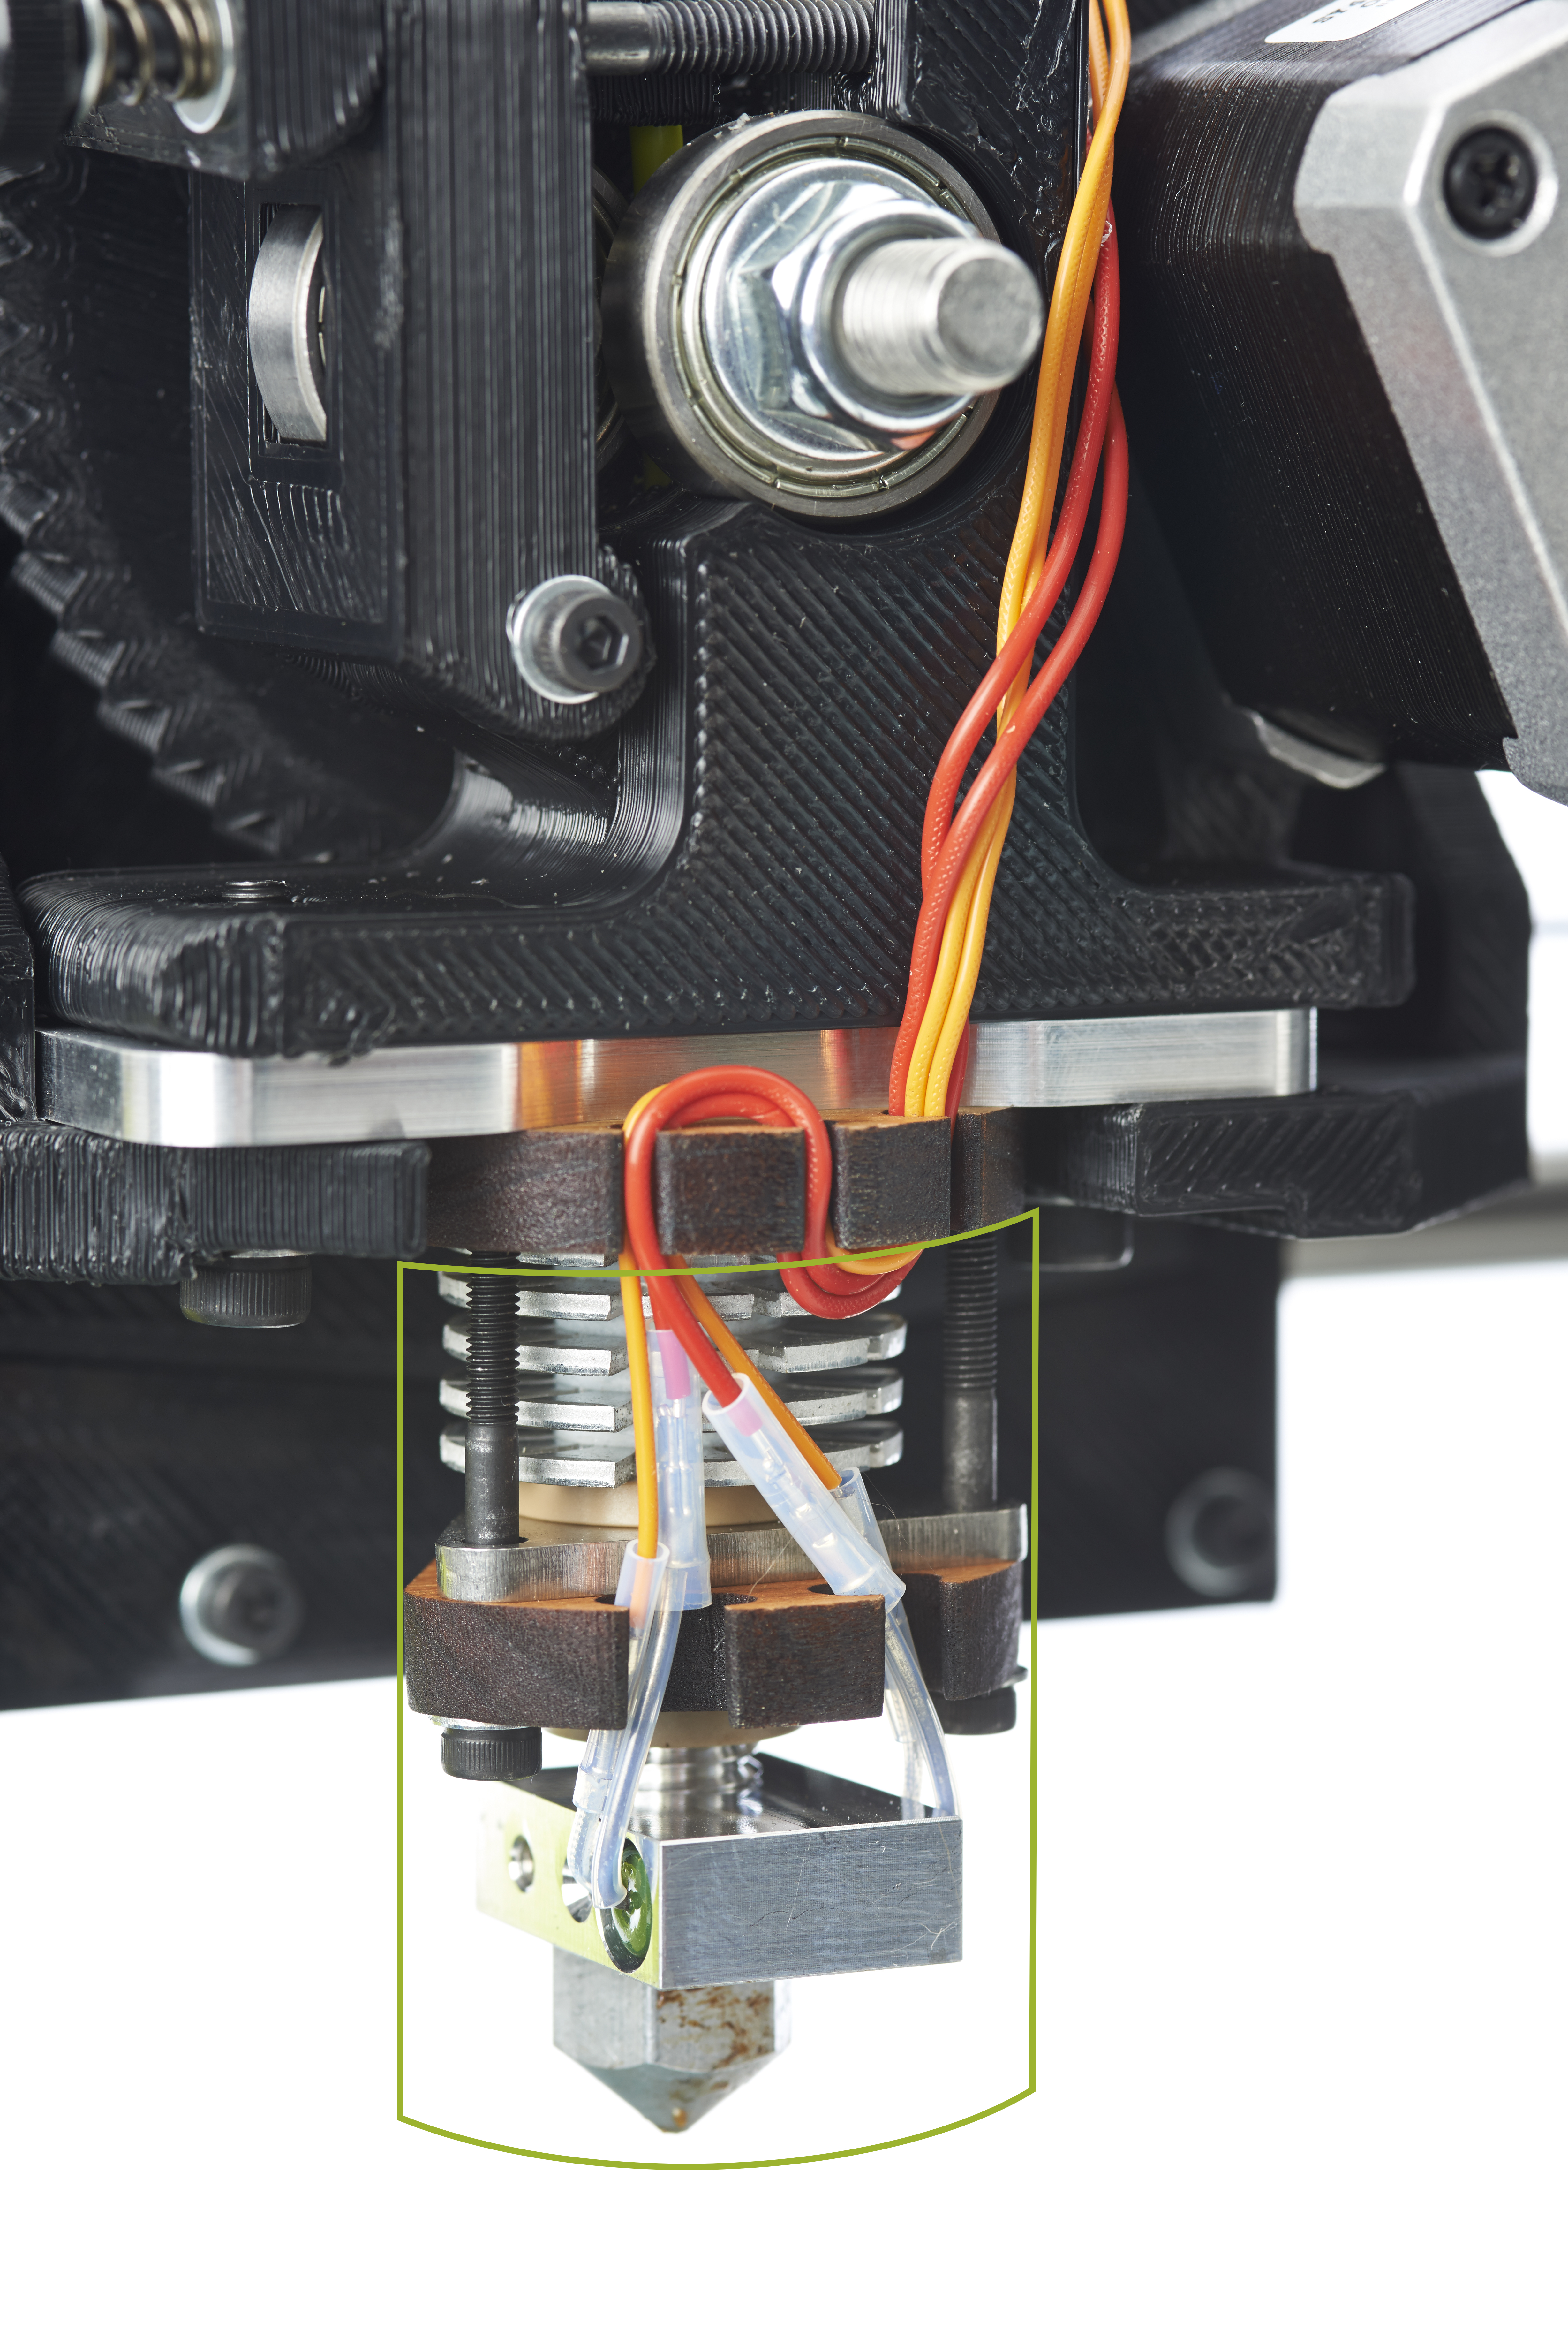
\includegraphics[width=0.5\textwidth]{simple_mode/extruder_clearance.JPG}
\caption{A diagram depicting the clearance around an extruder.}
\label{fig:a_diagram_depicting_extruder_clearance}
\end{figure}
% paragraph sequential_printing (end)


\subsubsection{Filament Settings}

The \texttt{Filament Settings} will normally be used infrequently, for example on receipt of a new roll of filament.

\begin{figure}[H]
\centering
\includegraphics[width=\textwidth]{simple_mode/simple_mode_filament_settings.png}
\caption{Simple Mode: Filament Settings.}
\label{fig:simple_mode_filament_settings}
\end{figure}

\paragraph{Filament.} % (fold)
\label{par:filament}
The \texttt{Diameter} setting will already have been filled from the value given during the wizard (see p.\pageref{sub:4_filament_diameter}), but can be updated here.

The \texttt{Extrusion multiplier} setting allows the fine tuning of the extrusion rate.  Whilst the value should ideally be set in the firmware it can be useful to test slight changes to the rate by altering this value.
% paragraph filament (end)

\paragraph{Temperature.} % (fold)
\label{par:temperature}
These values are also filled from the wizard, but here the opportunity exists to set the temperature for the first layer (see p.\pageref{sec:the_important_first_layer}).
% paragraph temperature (end)


\subsubsection{Printer Settings}

The \texttt{Printer Settings} will be updated the least, unless Slic3r is going to be used for many printers, for example, in a 3D printer farm.

\begin{figure}[H]
\centering
\includegraphics[width=\textwidth]{simple_mode/simple_mode_printer_settings.png}
\caption{Simple Mode: Printer Settings.}
\label{fig:simple_mode_printer_settings}
\end{figure}

\paragraph{Size and coordinates.} % (fold)
\label{par:size_and_coordinates}
The \texttt{Bed size} setting is taken from the wizard (see p.\pageref{sub:2_bed_size}), and the \texttt{Print center} is simply the mid-point of these values.  \texttt{Z offset} can be used to compensate for an incorrectly calibrated Z end-stop.  If the nozzle stops slightly too far from the bed, then adding a negative value will offset all layers by that amount.  The real solution however is to fix the end-stop itself.
% paragraph size_and_coordinates (end)

\paragraph{Firmware.} % (fold)
\label{par:firmware}
As selected in the wizard (see p.\pageref{sub:1_firmware_type}), \texttt{G-code flavour} defines the dialect of G-code generated.
% paragraph firmware (end)


\paragraph{Extruder.} % (fold)
\label{par:extruder}
\texttt{Nozzle diameter} was defined in the wizard (see p.\pageref{sub:3_nozzle_diameter}).
% paragraph extruder (end)

\paragraph{Retraction.} % (fold)
\label{par:retraction}
Unless the material being extruded has a very high viscosity it will ooze between extrusions due to gravity.  This can be remedied against by reducing the time between extrusions, and by actively retracting the filament between extrusions.  Setting the \texttt{Length} parameter to a positive value will cause the filament to be reversed by that many millimeters during travel.

Setting the \texttt{Lift Z} parameter to a positive value will raise the entire extruder on the Z axis by that many millimeters during each travel.  This can be useful to ensure the nozzle will not catch on any already laid filament.
% paragraph retraction (end)

\paragraph{Start G-code.} % (fold)
\label{par:start_g_code}
Custom gcode commands that run before the print run starts.  Some common gcodes to use are:
\begin{itemize}
	\item \textbf{G28}  - Homes all the axes.
\end{itemize}
The RepRap wiki is a good resource to learn about the variety of gcodes available: \texttt{http://reprap.org/wiki/G-code}.  

Note: Be sure to check that a given gcode is valid for your firmware.
% paragraph start_g_code (end)

\paragraph{End G-code.} % (fold)
\label{par:end_g_code}
Custom gcode commands that run after the print run ends.  Some common gcodes to use are:
\begin{itemize}
	\item \textbf{M104 S0}  - Sets the extruder temperature to zero.
	\item \textbf{M140 S60}  - Sets the heat bed temperature to sixty.
	\item \textbf{G28 X0} - Home the X axis.
	\item \textbf{M84}  - Disables the motors.
\end{itemize}
% paragraph end_g_code (end)
